\documentclass[12pt]{article}
\usepackage{tikz}
\usetikzlibrary{shapes,snakes}
\usetikzlibrary{arrows,automata}
\usepackage{algorithm}
\usepackage{algorithmic}
\usepackage{graphicx} 
\usepackage{fancybox}
\usepackage{setspace}  
\usepackage[colorlinks,linkcolor=blue,citecolor=magenta]{hyperref}
\usepackage{enumerate} 
\usepackage{amsthm,amssymb,amsmath}
\usepackage{indentfirst}
\usepackage{listings}
\usepackage{alltt}
\usepackage{clrscode}
\usepackage{float}
\renewcommand{\algorithmiccomment}[1]{// #1}
\floatstyle{plain}
\newtheorem{theorem}{Theorem}[section]
\newfloat{program}{h}{lop}[section]
\floatname{program}{}
\begin{document}

\title{Initial Value Computation}
\author{}
\date{\today}
\maketitle
\newcommand{\dom}{\textsf{dom}}
\newcommand{\arity}{\textsf{arity}}
\newcommand{\InputVars}{\textsf{InputVars}}
\newcommand{\OutputVars}{\textsf{OutputVars}}
\newcommand{\Rel}{\textsf{Rel}}
\newcommand{\Ext}{\textsf{Ext}}

\section{Defining domains}
\label{sec:definingdomains}
In this draft we want to explain the notion of domains in DBToaster calculus \cite{1}. DBToaster uses query language AGCA(which is stands for AGgregation CAlculus). 
AGCA expressions are built from constants, variables, relational atoms, aggregate sums (Sum), conditions, and variable assignments ($\gets$) using ``+''  and ``$\cdot$''. The abstract syntax can be given by the EBNF:
\begin{equation}
\label{def:agca}
q\text{ ::- }q\cdot q | q + q|v \gets q |v_{1}\theta v_{2}|R(\vec{y})|\text{c}|\text{v}|(M[\vec{x}][\vec{y}]\text{::-}q)
\end{equation}
The above definition can express all SQL statements. Here $v$ denotes variables, $\vec{x},\vec{y}$ tuples of variables, $R$ relation names, $c$ constants, and $\theta$ denotes comparison operations $(=,\neq, >, \geq, <, \text{ and }\leq)$.
 ``+'' represents unions and ``$\cdot$'' represents joins. Assignment operator($\gets$) takes an query and assigns its result to a variable($v$). A map $M[\vec{x}][\vec{y}]$ is a subquery with some input($\vec{x}$) and output($\vec{y}$) variables. It can be seen as a nested query that for the arguments $\vec{x}$ produces the output $\vec{y}$, it is not defined in \cite{1} but we added here for the purpose of this work.

The domain of a variable is the set of values that it can take. The domain of all the variables in a query expression can easily be computed recursively if some rules are respected. We will use through out the entire paper the notation of $\text{\dom{}}_{\vec x}(q)$ for the domain of a set of variables, where $q$ is the given query and $\vec x$ is a vector representing the variables(not necessarily present in the expression $q$). We will start by saying the $\vec x=\textless x_1,x_2,x_3,\cdots,x_n\textgreater$ will be the schema of all the variables 
and that $\vec c=\textless c_1,c_2,c_3,\cdots,c_n\textgreater$ will be the vector of all constants, that will match the schema presented by $\vec x$. It is not necessary that $\vec{x}$  has the same schema as the given expression. We will give the definition of $\dom{}_{\vec x}(R(\vec y))$:

%\begin{equation}
%\label{def:relation}
%\dom{}_{\vec x}(R(\vec y))=\bigg\{\vec %c\,\Big|\,(\prod_{i:x_{i}\in \vec y}^{}(x_{i}\gets %c_{i})\cdot R(\vec y))\not= 0\bigg\}
%\end{equation}

\begin{equation}
\label{def:relation}
\dom{}_{\vec x}(R(\vec y))=\bigg\{\vec c\,\Big|\,\sigma_{\forall x_i\in(\vec{y}): x_{i}=c_{i}}R(\vec y)\not= \const{NULL}\bigg\}
\end{equation}

Thus, we can evaluate $\text{\dom}_{\vec{x}}$ for a broader range of $\vec{x}$ and it is not restricted by the schema of the input query expression. In such cases the \dom{} is infinite as the not presenting variables in the query can take any value.

For the comparison operator ($v_{1}\theta v_{2}$), where $v_1$ and $v_2$ are variables, we can compute the domain as follows:
%\begin{equation}
%\text{\dom{}}_{\vec{x}}(v_{1}\theta v_{2})=\bigg\{\vec{c}\,\Big|\,\Big(\big(\prod_{i}(x_{i}\gets c_{i})\big)(v_{1}\theta v_{2})\Big)\not= 0\bigg\}
%\end{equation}

\begin{equation}
\text{\dom{}}_{\vec{x}}(v_{1}\theta v_{2})=\bigg\{\vec{c}\,\Big|\,\forall i,j:(v_{1}=x_{i}\land v_{2}=x_{j})\Rightarrow c_{i}\theta c_{j}\bigg\}
\end{equation}

The domain of a comparison is infinite.

For the join operator we can write:
\begin{equation}
\label{def:join}
\text{\dom{}}_{\vec{x}}(q_{1}\cdot q_{2})=\{\vec{c}\,|\vec{c}\in\text{\dom{}}_{\vec{x}}(q_{1})\land\vec{c}\in\text{\dom{}}_{\vec{x}}(q_{2})\}
\end{equation}
while for the union operator the domain definition is very similar:
\begin{equation}
\label{def:plus}
\text{\dom{}}_{\vec{x}}(q_{1}+ q_{2})=\{\vec{c}\,|\vec{c}\in\text{\dom{}}_{\vec{x}}(q_{1})\lor\vec{c}\in\text{\dom{}}_{\vec{x}}(q_{2})\}
\end{equation}
\begin{eqnarray}
\dom{}_{\vec x}(constant)=\Big\{\vec c\Big\}\label{def:const}\\
\dom{}_{\vec x}(variable)=\Big\{\vec c\Big\}\label{def:var}
\end{eqnarray}
In \eqref{def:const} and \eqref{def:var}  $\vec{c}$ stands for all possible tuples match schema of $\vec{x}$, so the domains in these two cases are infinite. 
Finally, we can give a formalism for expressing the domain of a variable that will participate in an assignment operation:
%\begin{equation}
%\label{assign1}
%\text{\dom{}}_{\vec{x}}(v\gets q_{1})=\bigg\{\vec{c}\,\Big|\vec{c}\in\text{\dom{}}_{\vec{x}}(q_{1})\land \bigg(\forall i:(x_{i}=v)\Rightarrow\Big(\big(q_{1}\cdot\prod_{j:x_{j}\neq v } (x_{j}=c_{j})\big)=c_{i}\Big)\bigg)\bigg\}
%\end{equation}
\begin{equation}
\label{assign2}
\text{\dom{}}_{\vec{x}}(v\gets q_{1})=\Big\{\vec{c}\Big|\vec{c}\in\text{\dom{}}_{\vec{x}}(q_{1})\land \big(\forall i,j: (x_{i}=v=x_{j})\Rightarrow(c_{i}=c_{j}=q_{1})\big)\Big\}
\end{equation}
In fact using implication operator in the above definition allows us to extend the $\vec{x}$ to whatever vector we want, as we already said the schema of $\vec{x}$ is not necessarily the same as the schema of $q$. %Here is a mathematical reformulation of \eqref{assign1}:
We can define the domain of a map(for map's definition refer to \cite{1}, \cite{2}) as follow:
\begin{equation}
\label{def:map}
\text{\dom}_{\vec{w}}(map[\vec{x}][\vec{y}])=\{\vec{c}|\vec{c}\in\text{\dom}_{\vec{w}}(\vec{x}\cup\vec{y})\}
\end{equation}
We define function \Ext{}  to extend(shrink) the schema of a domain, $a$ as input with schema $\vec{y}$:
\begin{equation}
\label{def:ext}
\text{\Ext}_{\vec{x}}(a_{\vec{y}})=\{\vec{c}|\sigma_{\forall i\,y_{i}\in\vec{x}:(y_{i}=c_{i})}a\neq \text{NULL}\}
\end{equation}
In \eqref{def:ext} we can consider $a$ as relation since it is a set and using the relational algebra on it. 
It is clear that if $\vec{x}\cap\vec{y}\neq\vec{x}$ it produces an infinite domain. 
\section{Defining arities}

\subsection{Definitions}

Having the definitions for the domains, we will try to give some insight regarding to the notion of arity. We will start with an example relation: $$q=R(a,b)\cdot S(b,c)$$ the schema for q will have three variables $(a,b,c)$. The arity of a tuple is the number of its occurrences in the relation, in other words the order of multiplicity of that tuple. The arity of a tuple will increase or decrease if insertions or respectively deletions will be made to a relation. For example:
\begin{table}[ht]
\centering
\begin{tabular}{c c c c}
	R & a & b & arity\\ [0.2ex]
	%heading
	\hline
	  & $\textless $1 & 2$\textgreater$ & 1 \\
	  & $\textless $1 & 3$\textgreater$ & 2 \\
	  & $\textless $3 & 4$\textgreater$ & 1 \\
\end{tabular}
\caption{Relation $R$}
\end{table}
\begin{table}[ht]
\centering
\begin{tabular}{c c c c}
	S & b & c & arity\\ [0.2ex]
	%heading
	\hline
	  & $\textless $1 & 1$\textgreater$ & 1 \\
	  & $\textless $2 & 2$\textgreater$ & 2 \\
	  & $\textless $3 & 5$\textgreater$ & 2 \\
\end{tabular}
\caption{Relation $S$}
\end{table}
\begin{table}[ht]
\centering
\begin{tabular}{c c c c c}
	$R\cdot S$ & a & b & c & arity\\ [0.2ex]
	%heading
	\hline
	  & $\textless $1 & 2 & 2$\textgreater$ & 2 \\
	  & $\textless $1 & 3 & 5$\textgreater$ & 4 \\
	  & $\textless $3 & 4 & $*\textgreater$ & 0 \\
	  & $\textless *$ & 1 & 1$\textgreater$ & 0 \\
\end{tabular}
\caption{Relation $R\cdot S$}
\end{table}

We need to maintain the maps for certain values as long as the arity of a tuple is greater then 0. If the arity  of the tuple drops to 0 then the tuple will not be taken into consideration and therefore it can be eliminated from the domains of the maps.

We need to store the arities inside each map and also way to compute the arity of an AGCA expression. Since we substitute the subexpressions with maps, we can easily consider the relations as the maps without input variables. Also a map with input variables can be seen as a relation with a group-by clause. Input variable of a map bind some variables. Thus if we compute the map values by all different combinations of these variables, we will look up into these values and return the appropriate value according to the input variables.  

We define the function \emph{arit} which will be used to compute the arity of a tuple in a certain relation. The function will be defined on the relation and the tuple for which the multiplicity order is desired to be computed. $$arit(\text{Relation } q,\text{Tuple } t)=\text{multiplicity order of }t\text{ in the } q =\pi_{t}(q)$$ where $\pi_{t}(q)$ means the projection of relation $q$ for the tuple $t$. This function can be used for the computation of the arity of the expressions from the AGCA: $q\text{ ::- }q\cdot q\text{ }|\text{ }q+q\text{ }|\text{ }q \theta t\text{ }|\text{ }t\gets q\text{ }|\text{ constant}\text{ }|\text{ variable}$. However constants and variables can be eliminated from the computation because relations are of interest.

\begin{align}
arit(q_{1}\cdot q_{2},t)&=\sum\limits_{\{t_{1}\}\Join \{t_{2}\}={t}}^{}arit(q_{1},t_{1})*arit(q_{2},t_{2})\\
arit(q_{1} + q_{2},t)&=arit(q_{1},t)+arit(q_{2},t)\text{, where Schema}(q_{1})\\=\text{Schema}(q_{2})\\
arit(v_1\text{ } \theta \text{ } v_2,t)&=\begin{cases}1,& \mbox{if } v_1\theta v_2 \mbox{ is true and }v_{1}\in t \land v_{2}\in t\\
0,& \text{otherwise} \mbox{ is false} 
\end{cases}\\
arit(v\gets q,t)&=\begin{cases}0, \mbox{ if $t\setminus\{v\}\not\in \text{\dom}_{Schema(t)}(q)$}\\ 1, \mbox{ otherwise} \end{cases}
\end{align}

\subsection{Extending the notion of domains to arities}

In the first part of the document we have talked about the definition of domains. Now we are going to talk about a combination between domains of tuples and the arities of those tuples. We can define something like the following:

$$\arity{}_{\vec x}(R(\vec y))=\bigg\{(\vec c,arit)\Big|\,\sigma_{\forall i:x_i\in\vec{y}\land x_{i}=c_{i}}R(\vec y)= arit \land arit \not= 0\bigg\}$$ 

The notion $\arity{}$ will help us construct both domains for each variable, but also compute the correct order of multiplicity of a tuple within a relation. If we have, for example, a relation $R$ with the following schema $R(\vec y=\textless x_1,x_2,\cdots,x_n\textgreater)$ and know that only a part of the variables defined by the schema are used for data flow to other relation $\vec x=\textless x_i,x_{(i+1)},\cdots,x_{(i+j)}\textgreater$, then the $\arity{}_{\vec x}(R(\vec y))$ will be all the groups of unique tuples with their order of multiplicity. This would be the same with having a query on relation $R$ with a group by using $\vec x$:
$$\mbox{SELECT }\vec{x} \mbox{,COUNT(*) FROM }R \mbox{ GROUP BY }\vec{x}$$
The query will produce a table with all the tuples and their arities. The tuples will be unique.

For example:

\begin{table}[H]
\centering
\begin{tabular}{c c c c c}
	R & a & b & c & d\\ [0.2ex]
	%heading
	\hline
	  & $\textless $1 & 2 & 4& 3$\textgreater$\\
	  & $\textless $2 & 3 & 5 & 4$\textgreater$\\
	  & $\textless $7 & 2 & 5 & 2$\textgreater$\\
	  & $\textless $6 & 3 & 9 & 4$\textgreater$\\
	  & $\textless $11 & 2 & 4 & 2$\textgreater$\\
	  & $\textless $1 & 2 & 9 & 3$\textgreater$\\
	  & $\textless $3 & 3 & 5 & 5$\textgreater$\\
	  & $\textless $3 & 2 & 5 & 2$\textgreater$\\
	  & $\textless $3 & 2 & 5 & 3$\textgreater$\\
\end{tabular}
\caption{Relation $R$}
\end{table}

In table 1 we have the relation $R$ with the schema $\vec y=\textless a,b,c,d\textgreater$. From that schema there are being used only two variables, $\vec x=\textless b,d\textgreater$ for the communication with other relation from a specific query. Applying the query presented in the previous paragraph we can compute all the unique tuples of $\vec x$ and their arities.

\begin{table}[H]
\centering
\begin{tabular}{c c c c}
	$\arity{}_{\textless b,d\textgreater}(R)$ & b & d & arit \\ [0.2ex]
	%heading
	\hline
	  & $\textless $2 & 3$\textgreater$ & 3\\
	  & $\textless $3 & 4$\textgreater$ & 2\\
	  & $\textless $2 & 2$\textgreater$ & 3\\
	  & $\textless $3 & 5$\textgreater$ & 1\\
\end{tabular}
\caption{Relation $R$}
\end{table}

Taking into account the rule defined for the computation of the $\arity{}$, we are going to have for relation $R$ the following:
$$\arity{}_{\textless b,d\textgreater}(R(\textless a,b,c,d\textgreater))=\{((2,3),3),((3,4),2),((2,2),3),((3,5),1)\}$$

So far we have explained only one type of expression in the AGCA: the simple relation $R(\vec y)$, however AGCA presents many more types. Therefore we have to explain each of other types of expression. We remind that in AGCA an expression q may be of the following form:
\begin{equation}
q\text{ ::- }q\cdot q | q + q|v \gets q |v_{1}\theta v_{2}|R(\vec{y})|\text{c}|\text{v}|(M[\vec{x}][\vec{y}]::-q)
\end{equation}
Exactly as we did with the definitions for the domains, we can write the definitions for the arities just extending the definition of the domain. For $q\text{::-}v_{1}\theta v_{2}$:
\begin{equation}
\text{\arity{}}_{\vec{x}}(v_{1}\theta v_{2})=\bigg\{(\vec{c},arit)\,\Big|\,\forall i,j:(v_{1}=x_{i}\land v_{2}=x_{j})\Rightarrow (c_{i}\theta c_{j}=arit)\bigg\}
\end{equation}
For $q\text{::-}q_{1}\cdot q_{2}$:
\begin{align} 
\text{\arity}_{\vec{x}}(q_{1}\cdot q_{2})=\big\{(\vec{c},arit)\,\big|(\vec{c},arit_{1})\in&\text{\arity}_{\vec{x}}(q_{1})\nonumber\\\land (\vec{c},arit_{2})\in\text{\arity{}}_{\vec{x}}(q_{2})& \land arit= arit_{1}\times arit_{2}\big\}
\end{align}
For $q\text{::-}q_{1}+q_{2}$:
\begin{align}
\text{\arity{}}_{\vec{x}}(q_{1}+ q_{2})=&\{(\vec{c},arit)\,|((\vec{c},arit_{1})\in\text{\arity{}}_{\vec{x}}(q_{1})\lor(\vec{c},arit_{2})\in\text{\arity{}}_{\vec{x}}(q_{2})) \nonumber\\&\land arit=arit_{1}+arit_{2}\}
\end{align}
For $q\text{::-}t\gets q$:
\begin{align}
\text{\arity{}}_{\vec{x}}(v\gets q)=\Big\{(\vec{c},arit)\Big|\vec{c}\in\text{\dom{}}_{\vec{x}}(q)\land \bigg(\Big(\big(\forall i: (x_{i}=v) & \nonumber\\\Rightarrow(c_{i}=q)\big)\land (arit=1)\Big)\lor (arit=0)\bigg)\Big\}
\end{align}

\section{Domain computation}

We are trying to compute the domain of variables that appear in queries. This computation is performed on the parse tree. We can traverse the tree in post order, first visiting the leaves that are represented by some relations and afterwards visiting the parent nodes and combining the relations of the children nodes. Using this technique we are trying to compute the domains, but also the vector $\vec x$ of all the variables defined in that query.

The intuition behind the algorithm is simple. For computing the domain of a node we first compute the domain of its left child and according to the operator of the node itself we decide how to send the information from left child to right child, and then the domain of the right child.

The algorithm needs as inputs the root of the tree and a structure that must be previously defined and returns a structure that contains the vector of variables($\vec{x}$) and the domains for each variable defined in the vector(\dom). This structur is called $NodeAttribute$ and it looks like:

\begin{program}
\begin{alltt}
struct \{
x: the vector of all the variables 
dom: the domains of all the variables
\}
\end{alltt}
\caption{$NodeAttribute$}
\label{struct}
\end{program}
In Algorithm \ref{alg1} we define function \textsf{computeDomain} which helps us to compute the domains for variables within a given query. When invoking the function, we pass as arguments of the function, the root of the parse tree and a structure which will have the vector of variables and the domain of the variables as nil, \textsf{computeDomain}$(root,s)$.
\par
In Algorithm~\ref{alg1} we have a variable $node$ which represents a node in the parse tree. It has 2 children which can be accessed by fields $left, right$. Also each node has a type field, which can be accessed by $type$. A type of a node can be any of different types in definition~\eqref{def:agca}. For handling map types we suppose that each node that represents a map has a child (accessible via filed $child$, line~\ref{lst:child}) which points to the map itself (i.e. Figure~\ref{fig:map}). In other words each map introduces an intermediate node in the tree structure, this node has two fileds $\vec{x},\vec{y}$ to represent input and output domain of the map. 

\begin{algorithm}[H]
\caption{computeDomains($node$,$s$)} 
\label{alg1}
\textbf{Input:} $node$ as the root of the tree to be traversed, and $s$ is of type $NodeAttribute$ \\
\textbf{Output:}  $result$ of type $NodeAttribute$ that contains vector of variables $\vec x$ and the domains of each variable $\dom{}_{\vec x}(query)$
\begin{algorithmic}[1]
\IF{$node.type=$``+''}
\STATE  $s_{1}\gets$ computeDomain($node.left, s$)
\STATE  $s_{2}\gets$ computeDomain($node.right, s$)
\STATE  $result.\vec{x}\gets s_{1}.\vec{x} \cup s_{2}.\vec{x}$ %\COMMENT{this will compute the vector for all the variables, both from the right and left node}
\STATE  $result.dom\gets \text{\dom}_{result.\vec x}(s_{1}.dom)\cup\text{\dom}_{result.\vec x}(s_{2}.dom)$
\ELSIF{$node.type=$``*''}
\label{line:join1}
\STATE  $s_{1} \gets \text{computeDomain}(node.left, s)$\label{line:join2}
\STATE $result\gets$ computeDomain$(node.right, s_{1})$
\ELSIF{$node.type=$``Map''}
\label{lst:map}
\STATE $node.\vec{x}\gets\text{\dom}_{s.\vec{x}}(s.dom)$
\STATE $node.\vec{y}\gets$computeDomain$(node.child,s)$\label{lst:child}
\STATE $result.\vec{x}\gets s.\vec{x}$
\STATE $result.dom\gets node.\vec{y}$
\ELSE 
\label{line10}
\STATE $result.\vec{x}\gets s.\vec{x} \cup \{\text{Var$(node)$}\}$\label{lst:setofallvar}
\STATE $result.dom\gets \text{\Ext}_{result.\vec{x}}(s.dom)\cap\text{\dom}_{result.\vec{x}}(node)$\label{line2}
\ENDIF
%\IF{$node.isMap=$ \TRUE}
%\STATE $Maps[node].\vec{x}\gets\text{\dom}_{\vec{x}}(s.dom)$
%\STATE $Maps[node].\vec{y}\gets result$
%\ENDIF
\RETURN $result$
\end{algorithmic}
\end{algorithm}
The order of Algorithm \ref{alg1} is $O(n\cdot P)$ where $n$ is the number of nodes in the parse tree and $P$ is the time needed for any rule of \dom{}'s computation, according to previous section. Clearly this algorithm visits each node only one time. \par

Algorithm \ref{alg1} all types of nodes: union nodes, join nodes, map nodes and all other type of nodes. In addition to nodes, we have three types of leaves: simple relations $R(\vec y)$, inequalities $v_{1}\theta v_{2}$ and assignment relations $v \gets q$. A union node or a join node will always have two children, therefore the line \ref{line10} will be executed when a leaf is visited. When a map node is encountered, line~\ref{lst:map}, then the algorithm should produce the domain of input and output variables. In line \ref{line2} we use function \Ext{} to extend the schema of the input domain to a broader schema of $result.\vec{x}$. We use this for extending a domain regarding to a new schema vector $result.\vec x$. 

In line~\ref{lst:setofallvar} we want to compute the set of variables in the node. Since the node is a leaf, it can represents a relation, an assignment or a comparison. We can compute the set of variables in a leaf with the following rules:
\begin{align}
\text{Var}(R(\vec{y}))&=\{y_{1},\cdots,y_{n}\}\\
\text{Var}(v_{1}\theta v_{2})&=\{v_{1},v_{2}\}\\
\text{Var}(v\gets q_{1})&=\{v\}\cup\text{Var}(q_{1})
\end{align}
\begin{figure}[htbp]
\begin{center}
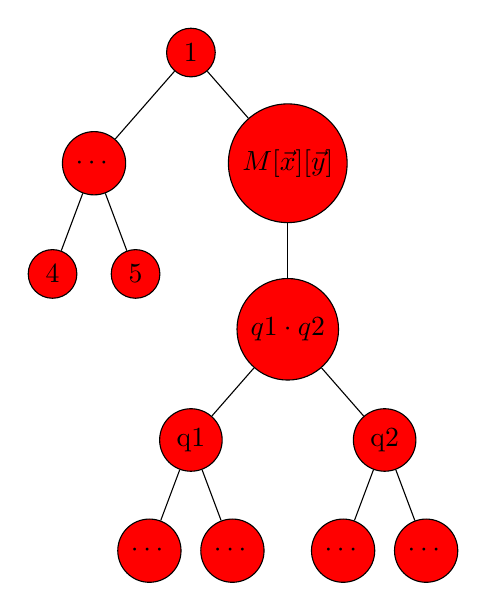
\begin{tikzpicture}%[level/.style={sibling distance=40mm,level distance=15mm}]
[level 1/.style={circle, draw,scale=1.0, fill=red,
    level distance=40pt, sibling distance=70pt},
    level 2/.style={circle, draw, scale=1.0,
    level distance=60pt, sibling distance=70pt},
    level 3/.style={circle, draw, scale=1.0,
    level distance=40pt, sibling distance=70pt},
    level 4/.style={circle, draw, scale=1.0,
    level distance=40pt, sibling distance=30pt}]
    \tikzstyle{every node}=[circle,draw,fill=red]
    \node[] (a){1}
        child { 
            node [](b){$\cdots$}
            child[sibling distance=30pt,level distance=40pt]{
            	node{4}
            }
            child[sibling distance=30pt,level distance=40pt]{
            	node{5}
            }
        }
        child{ 
        		node[](c){$M[\vec{x}][\vec{y}]$}
        		child{
        			node[](d){$q1\cdot q2$}
        			child{
        				node[](f){q1}
        				child{node[](g){$\cdots$}}
        				child{node(h){$\cdots$}}
        				}
        			child{
        				node[](i){q2}
        				child{node[](j){$\cdots$}}
        				child{node(k){$\cdots$}}
        				}
        			}
		};
\end{tikzpicture}
\end{center}
\caption{Tree representation}
\label{fig:map}
\end{figure}

%\begin{figure}[htbp]
%\begin{center}
%\begin{tikzpicture}%[level/.style={sibling distance=40mm,level distance=15mm}]
%[level 1/.style={circle, draw,scale=1.0, fill=red,
%    level distance=30pt, sibling distance=100pt},
%    level 2/.style={circle, draw, scale=1.0,
%    level distance=50pt, sibling distance=60pt}]
%    \tikzstyle{every node}=[circle,draw,fill=red]
%    \node[] (a){1}
%        child { 
%            node [](b){2}
%            child{node(d){4}}
%            child{node(e){5}} 
%        }
%        child { 
%        		node[] (c){3}
%		child{node[](f){6}}
%		child{node(g){7}}
%	};
%	\draw[->] (a) to [bend right=25](b);
%	\draw[->] (b) to [bend right=25](a);
%	
%	\draw[->] (a) to [bend right=25](c);
%	\draw[->] (c) to [bend right=25](a);
%	
%	\draw[->] (b) to [bend right=25](d);
%	\draw[->] (d) to [bend right=25](b);
%	\draw[->] (b) to [bend right=25](e);
%	\draw[->] (e) to [bend right=25](b);
%	\draw[->] (c) to [bend right=25](f);
%	\draw[->] (f) to [bend right=25](c);
%	\draw[->] (c) to [bend right=25](g);
%	\draw[->] (g) to [bend right=25](c);
%	
%\end{tikzpicture}
%\end{center}
%\caption{Tree traversal}
%\label{fig1}
%\end{figure}
The algorithm starts with node 1, which represents the root of the parse tree. It recursively goes through each of the leaves, therefore constructs the variable vector and also the domain for each variable.
%It is known that the left most leaf will always be a relation that produces only output variables. Otherwise, if this condition is not sustained then it will contradict the rules imposed by the DBToaster calculus. Therefore node 4 will always be a simple relation that will give some output variables, which may help in future nodes if those nodes have input variables. If, for example node 5 will have input variables, then those variables will depend only on the output variables that node 4 is giving.
	
We have mentioned that besides map nodes, there are two more types of intermediate nodes: the union node and the join node. When a union node is met, then it is known that domains of variables will not pass over this operator and for that the variables and their domains, which were obtained in the parent, will be passed to each of this node's children. Thus it applies the distribution rule of the join operator over the union operator. For example if we have $ q1 * (q2 * q3 + q4 * q5) \equiv q1 * q2 * q3 + q1 * q4 * q5$, the variables and domain obtained for $q1$ will be passed both to $q2*q3$ and $q3*q4$, without modifying any of the domains, regarding that some domains may change on one branch, for example $q2*q3$. For the other type of node, the join node, the passing of domains is allowed, and therefore a domain can be refined by the relation on the right side of the parent node.
	
	Every time the algorithm encounters a map then it will create the domain for that specific map. Here we can make a difference between input and output variables, because the domain of input variables is dependent on the domains of output variables from the left side of the map's parent node, and the domain of the output variables are going to be produced by the children of the map's node. %All this information will be stored in a global variable which can be easily accessed.

A node which is represented by a map will have only one child, because as we mentioned in the definition of the AGCA expression, a map can be defined over an expression or expressions: $M[\vec{x}][\vec{y}]\text{::-}q$
\begin{theorem}
Algorithm \ref{alg1} computes the domain of each variables and maps.
\end{theorem}

\begin{proof}
The proof is by induction on the height of the tree. The theorem is held for a tree consisting of only one node. Since this node is a simple relation and the Algorithm \ref{alg1} goes  through lines \ref{line10}-\ref{line2}. As we defined, the domain of any empty set is infinite(all possible values) so the domain is correctly computed in line \ref{line2}.

Now suppose that the Algorithm \ref{alg1} works for all the trees of a height less than $k$. We want to prove that it will work as well for trees of height $k$. Let $T$ be a tree with height $k$. If root represents a map, it has a child and we correctly computed its output domain, so the same is held for the map itself and the theorem follows in this case. Otherwise
the root should have two children. The height of both of these children should be less than $k$. So we have correctly compute the domain of the left child and its input variable. Now we have two cases, if the root node is a union node or a join node. If this is a union node then we can compute the domain of the right child independently, since no information is passed over the ``+'' in DBToaster\cite{1}. We compute the domain of the root according to definition \eqref{def:plus}. But if the root node is a join node, we have to pass the information from left child to the right child, since the right child may have some input variables which are defined in the left child. This is done in lines \ref{line:join1},\ref{line:join2}.\par
Thus in either of two cases we compute the domain of the root correctly and the theorem follows.
\end{proof}

\section{Arity computation}

We have defined some rules for the computation of the domains and the arities of each tuple. Having them, we can start writing an algorithm to compute the domains and the tuples' arities. We will start with the algorithm that will compute the domains and arities for each element. The algorithm will be similar to the algorithm that we have written for determining only the domains of variables that appear within a query.

As the algorithm presented for the computation of the domains, this one must have as well a structure which will help in the computation.

\begin{program}
\begin{alltt}
struct \{
x: the vector of all the variables 
arity: the domain and arities of all the variables
\}
\end{alltt}
\caption{$nodeArityAttribute$}
\label{struct}
\end{program}
%We define three new elements that help us in the arity computation. These elements will be connected with the schema of the vector of variables. We know that $\vec x$ will represent all the names of the variables that are being used to compute in the previous section the domain, and now is being used to compute the arities. Therefore the vector of variables will have the following form: $\vec x = \textless x_1,x_2,\cdots,x_n\textgreater$. We are concerned by the schemas for the join operation because the arities will be defined by the common variables of the schema of different relations.
%
%We have $q\text{::-}q_{1} \cdot q_{2}$, where $q_{1}$ will have the schema $\vec x=\textless x_1,x_2,\cdots,x_n\textgreater$ and $q_{2}$ will have the schema $\vec y=\textless y_1,y_2,\cdots y_m\textgreater$ ($m$ is not necessarily equal to $n$). We define the common schema between relation $q_{1}$ and $q_{2}$: $\vec z=\textless z_1,z_2,\cdots z_p\textgreater$, and the differences between schemas: first the elements that appear in $q_{1}$ but do not appear in $q_{2}$: $\vec w_{1}=\textless w_{11},w_{12},\cdots w_{1r}\textgreater$ and second the elements that appear in $q_{2}$ and do not appear in $q_{1}$: $\vec w2=\textless w_{21},w_{22},\cdots w_{2s}\textgreater$; we will have $p+r=n$ and $p+s=m$.
%
%We are going to have from the first the following: $$\arity{}_{\vec x}(q_{1})=\{(\vec c,arit)| \forall \vec c \mbox{ and their arit, that characterize expression $q_{1}$}\}$$. 
%For the expression $q_{2}$ we are going to have a similar set of elements $$\arity{}_{\vec y}(q_{2})=\{(\vec c,arit)| \forall \vec c \mbox{ and their arit, that characterize expression $q_{2}$}\}$$. 
%We are going to extract an element from $\arity{}_{\vec x}(q_{1})$, $(\vec{c_{1}},arit_{1})\in\arity{}_{\vec x}(q_{1})$, and an element from the second set $\arity{}_{\vec y}(q_{2})$, 
%$(\vec{c_{2}},arit_{2})\in\arity{}_{\vec y}(q_{2})$.
%
%We are going to define a function $f$, which will be defined on a vector of values having a schema and will produce a vector of values that will have a given schema. 
%$$f_{\mbox{schema for the vector}}:\textless val_1,\cdots,val_l\textgreater \rightarrow \textless val'_1,\cdots,val'_k\textgreater$$
%
%For example we will have $(\vec{c1},arit1)$ from q1 with schema $\vec x$ and $(\vec{c2},arit2)$ from q2 with schema $\vec y$. We want to compute the vector of values that has the schema of the common schema of the two relations $\vec z$. Therefore we will have for $q1$: $f1=f_{\vec{z}}(\vec{c1})$ and for $q2$: $f2=f_{\vec{z}}(\vec{c2})$. If $f1==f2$ then the join operation for the two relations match and the arities for the bigger tuple of variables will the product between arit1 and arit2.
%
%The expression $q1\cdot q2$ will have the following tuple : $$\textless w_{11},w_{12},\cdots w_{1r},z_1,z_2,\cdots z_p,w_{21},w_{22},\cdots w_{2s}\textgreater$$ and the arity of this tuple will be $arit1 * arit2$ if the relation explained the previous paragraph holds.
Algorithm~\ref{alg3} is similar to the Algorithm~\ref{alg1}. The steps are the same, we traverse the parse tree, seeking all the nodes and test them to find out the type. The basic mechanism is the same when talking about reaching a node that will be a union node or a join node or even a map node. The difference will appear at the results presented, because in  Algorithm~\ref{alg1} we will compute only domains of each tuple, whilst in Algorithm~\ref{alg3} we will compute the combination between the domains and the arity of each tuple inside the domains. 
\begin{algorithm}[H]
\caption{computeArities($node$,$s$)} 
\label{alg3}
\textbf{Input:} $node$ as the root of the tree to be traversed, and $s$ which is of type $nodeArityAttribute$ \\
\textbf{Output:}  $result$ of type $nodeArityAttribute$ that contains vector of variables $\vec x$ and the domains of each variable with arities
\begin{algorithmic}[1]
\IF{$node.type=$``+''}
\STATE  $s_{1}\gets$ computeArities($node.left, s$)
\STATE  $s_{2}\gets$ computeArities($node.right, s$)
\STATE  $result.\vec{x}\gets s_{1}.\vec{x} \cup s_{2}.\vec{x}$
\STATE  $result.\arity{}\gets \{(\vec{c},arit)|(\vec{c_{1}},arit_{1})\in s_{1}.\arity{}\land (\vec{c_{2}},arit_{2})\in s_{2}.\arity{}\land (\vec{c_{1}}=\vec{c_{2}}\Rightarrow (\vec{c},arit)=(\vec{c_{1}},arit_{1}+arit_{2}))\land (\vec{c_{1}}\not=\vec{c_{2}}\Rightarrow (\vec{c},arit)=(\vec{c_{1}},arit_{1})\lor (\vec{c},arit)=(\vec{c_{2}},arit_{2}) )\}$
\ELSIF{$node.type=$``*''}
\STATE  $s_{1} \gets \text{computeArities}(node.left, s)$
\STATE $result\gets \text{computeArities}(node.right, s_{1})$
\ELSIF{$node.type=$``Map''}
\STATE $node.\vec{x}\gets s.\arity{}$
\STATE $s_{1}\gets\text{computeArities}(node.child,s)$
\STATE $node.\vec{y}\gets s_{1}.\arity{}$
\STATE $result.\vec{x}\gets s_{1}.\vec{x}$
\STATE $result.\arity{}\gets node.\vec{y}$
\ELSE 
\STATE $result.\vec{x}\gets s.\vec{x} \cup \{\text{Var$(node)$}\}$
\STATE $aux \gets extendAritiesToSchema_{result.\vec{x}}(s.\arity{})$
\STATE $result.\arity{}\gets \{(\vec{c},arit)|(\vec{c},arit_{1})\in aux\land (\vec{c},arit_{2})\in \arity{}_{result.\vec{x}}(node) \land (arit=arit_{1}*arit_{2}) \}$
\ENDIF
%\IF{$node.isMap=$ \TRUE}
%\STATE $Maps[node].\vec{x}\gets\text{\dom}_{\vec{x}}(s.dom)$
%\STATE $Maps[node].\vec{y}\gets result$
%\ENDIF
\RETURN $result$
\end{algorithmic}
\end{algorithm}


\section{Maintaining the domains using arities}

The main goal is to maintain the domains of the variables of each map that are presented in query expression. We give a solution of maintaining these domains, see how the domains will increase or decrease if tuples are being added or deleted from the relations.

\begin{theorem}
The arity of a tuple in the domain of a simple relation will always be greater than 0.
\end{theorem}

Having this algorithm we can compute now the combination between the domain and the arities of the tuples that compose the domain. The algorithm should traverse the parse tree until it reaches the leaf that represents the relation that needs an update. Therefore a Depth First Algorithm can be used. First we shall talk about inserting a new tuple to an existing relation. When a leaf with the specified relation is encountered, we check if the tuple already exists in the set of arities. If the tuple exists, then we will retrieve the arity, and just for the fact that it exists in the domain of a relation the arity will be greater than 0. We increment the arity and repack everything and put it back in the set. If the tuple is not found in the domain of the relation that means that we will have a transition of the arity from $0 \rightarrow 1$, because we have to add the tuple to the existing domain, and therefore we have to recompute the domains for each and every map starting from that leaf.\\\par
When talking about making a deletion of a tuple inside a relation, most of the algorithm will remain the same. We should first find the leaf that represents the designated relation, find if the tuple is or is not inside the domain of the relation. If the tuple is not inside the domain then there appears an error because you can not delete something from the table of database without that tuple appearing inside the table. Therefore the tuple that is going to be deleted must appear in the domain of the relation. Having the group (domain,arity) we can test the arity. If the arity, after deleting the tuple, remains greater than 0 then the algorithm stops by making the modification to the arity, packing the results and putting it back into the set of the domain. Otherwise, if the arity drops to 0, then we will have a transition of $1 \rightarrow 0$ and thus we have to recompute each and every domain of the maps starting from the leaf that suffered a change.\\\par
To conclude the small description of the algorithm, we are interested only in transitions $0 \rightarrow 1$ or $1 \rightarrow 0$, because only then we will have to recompute every domain of the maps.

A sketch of the algorithm would look like as follows:

\begin{algorithm}[H]
\caption{maintainDomains($node$,$(tuple,arity)$,$name_{relation}$)} 
\label{alg2}
\textbf{Input:} the root of the parse tree, the tuple that needs to be added with arity 0 (at first), the name of the relation \\
\textbf{Output:} the algorithm would not output nothing because it will produce the necessary changes along it goes
\begin{algorithmic}[1]
\STATE
\end{algorithmic}
\end{algorithm}

\subsection{Incrementally Maintaining For Insertion and Deletion}
In this section we give an algorithm for computing the domains incrementally after each deletion or insertion. Let $T$ be the parse tree as we had in the previous sections. We want to know how the domain of each node changes with any insertion or deletion from any relations. If the domain of any leaves of $T$ changes, in the worst case we need to reevaluate domains of all the nodes in $T$. For an example, suppose the leftmost leaf changes and all other leaves depends on it, like $R(\vec{y})\cdot\prod_{i}{(y_{i}>a_{i})}$ where $a_{i}$ are constants.
Although in the worst case we need to reevaluate the domains of all nodes, but in some cases we can have some optimization in order to avoid recomputing the domains. We define function \InputVars{} to a function that takes a node and returns its input variables. We can define a similar function \OutputVars{} for output variables.
\begin{align}
\text{\InputVars}(R(\vec{y}))&=\{\}\\
\text{\InputVars}(v_{1}\theta v_{2})&=\{v_{1},v_{2}\}\\
\text{\InputVars}(q_{1}+q_{2})&=\text{\InputVars}(q_{1})\cup\text{\InputVars}(q_{2})\\
\text{\InputVars}(q_{1}\cdot q_{2})&=\text{\InputVars}(q_{1})\cup\text{\InputVars}(q_{2})-\text{\OutputVars}(q_{1})\\
\text{\InputVars}(v\gets q_{1})&=\text{\InputVars}(q_{1})\\
\text{\OutputVars}(R(\vec{y}))&=\vec{y}\\
\text{\OutputVars}(v_{1}\theta v_{2})&=\{\}\\
\text{\OutputVars}(q_{1}+q_{2})&=\text{\OutputVars}(q_{1})\cap\text{\OutputVars}(q_{2})\\
\text{\OutputVars}(q_{1}\cdot q_{2})&=\text{\OutputVars}(q_{1})\cup\text{\OutputVars}(q_{2})\\
\text{\OutputVars}(v\gets q_{1})&=\{v\}
\end{align}
According to the above definitions we can give an algorithm for computing the changes to each map for any insertion or deletionXXXX. For our purpose we need a way to show the set of relations contains in each node, we show this by \Rel{} and define it as follow:
\begin{align}
\text{\Rel}(R(\vec{y}))&=R\\
\text{\Rel}(v_{1}\theta v_{2})&=\{\}\\
\text{\Rel}(q_{1}+q_{2})&=\text{\Rel}(q_{1})\cup\text{\Rel}(q_{2})\\
\text{\Rel}(q_{1}\cdot q_{2})&=\text{\Rel}(q_{1})\cup\text{\Rel}(q_{2})\\
\text{\Rel}(v\gets q_{1})&=\text{\Rel}(q_{1})
\end{align}

\begin{algorithm}
\caption{CheckRightNode($node,v_{1},R,s$)}
\label{alg:sub}
\textbf{Input:} $node$ as the root of the tree to be traversed, $v_{1}$ a flag indicating if the left subtree has changed, $R$ the relation to be modified and $s$ as the structure \\
\textbf{Output:} A pair whose first element is a boolean to indicate if any domains in the subtree rooted at $node.right$ has changed
and the second element is the \dom($node.right$)
\begin{algorithmic}[1]
\IF{$R\in$\Rel($node.right$) \OR $(v_{1}=\text{\TRUE}$   \AND \OutputVars $(node.left)\cap$ \InputVars $(node.right)\neq\emptyset$ )}
\RETURN MaintainDomains$(node.right,R,s)$
\ELSE
\RETURN (\FALSE$,node.right.s)$
\ENDIF
\end{algorithmic}
\end{algorithm}
\begin{algorithm}
\caption{MaintainDomains$(node,R,s)$}
\label{alg:MD}
\textbf{Input:} $node$ as the root of the tree to be traversed, $R$ the relation to be modified and $s$ as the structure \\
\textbf{Output:} A pair whose first element is a boolean to indicate if any domains in the subtree rooted at $node$ has changed
and the second element is the \dom($node$)
\begin{algorithmic}[1]
\IF{$R\in$\Rel(node.left)}
\label{lst:ml1}
\STATE $(v_{1},s_{1})\gets \text{MaintainDomains($node.left,R,s$)}$
\ELSE
\STATE $(v_{1},s_{1})\gets (\FALSE,node.left.s)$
\ENDIF
\label{lst:ml2}
\IF{$node.type=$``+''}
\STATE $(v_{2},s_{2})\gets$CheckRightNode$(node,v_{1},s)$
\STATE  $node.s.dom\gets \text{\dom}_{node.s.\vec x}(s_{1}.dom)\cup\text{\dom}_{node.s.\vec x}(s_{2}.dom)$
\ELSIF{$node.type=$``*''}
\STATE $(v_{2},node.s.dom)\gets$CheckRightNode$(node,v_{1},s_{1})$
\ELSIF{$node.type=$``Relation''}
\STATE Apply changes to the relation if it is $R(\vec{y})$ and set $v_{2}$ \TRUE{} if the domain changed
\STATE $node.s.dom\gets\text{\dom}_{node.s.\vec{x}}(node)$
\ELSIF{$node.type=$``Map''}
%\label{lst:map}
\STATE $node.\vec{x}\gets\text{\dom}_{s.\vec{x}}(s.dom)$
\STATE $(v_{2},node.\vec{y})\gets$MaintainDomains$(node.child,R,s)$%\label{lst:child}
\STATE $result.\vec{x}\gets s.\vec{x}$
\STATE $result.dom\gets node.\vec{y}$
\ELSE
\STATE $node.s.dom\gets \text{\dom}_{node.s.\vec{x}}(s.dom)\cap\text{\dom}_{node.s.\vec{x}}(node)$%\label{line2}
\STATE $v_{2}\gets \FALSE$
\ENDIF
\RETURN $(v_{1}\OR\,v_{2},result)$
\end{algorithmic}
\end{algorithm}
The intuition of Algorithm~\ref{alg:MD} is simple. Suppose we want to modify relation R(insertion or deletion). In each node we first check whether the left subtree contains $R$ or not. If so, we continue recursively in the left subtree(lines \ref{lst:ml1}-\ref{lst:ml2}). We run the algorithm on the right subtree if and only if it contains $R$ or the left subtree has changed due to the modification and the right subtree has some input variables which depend on the output variables of the left subtree. Deciding whether or not to run the algorithm on the right subtree is preformed by Algorithm~\ref{alg:sub}.
According to the type of nodes, as we had in Algorithm~\ref{alg1}, we compute the domain of $node$. Here we suppose that each node has a left and right child as before and structure $s$ as defined in \ref{struct}. We suppose that before any executions of Algorithm~\ref{lst:ml2}, Algorithm~\ref{alg1} has been executed at least one time. So for each $node$ we have associated a structure $s$. Thus with $s$ we can access to the domain($dom$) of each node and the set of its variables($\vec{x}$). 

\begin{thebibliography}{9}
\bibitem{1} C. Koch, \emph{Incremental Query Evaluation in a Ring of Databases},  preprint (2011).
\bibitem{2} O. Kennedy, Y. Ahmad, C. Koch. \emph{DBToaster: Agile views for a dynamic data management system}. In CIDR, 2011.
\end{thebibliography}
\end{document}




